In this chapter the basic concepts of process mining, text mining, supervised learning, long short-term memory networks are presented. Furthermore, formal definitions and notations are introduced.


%\begin{figure}
	%\centering
	%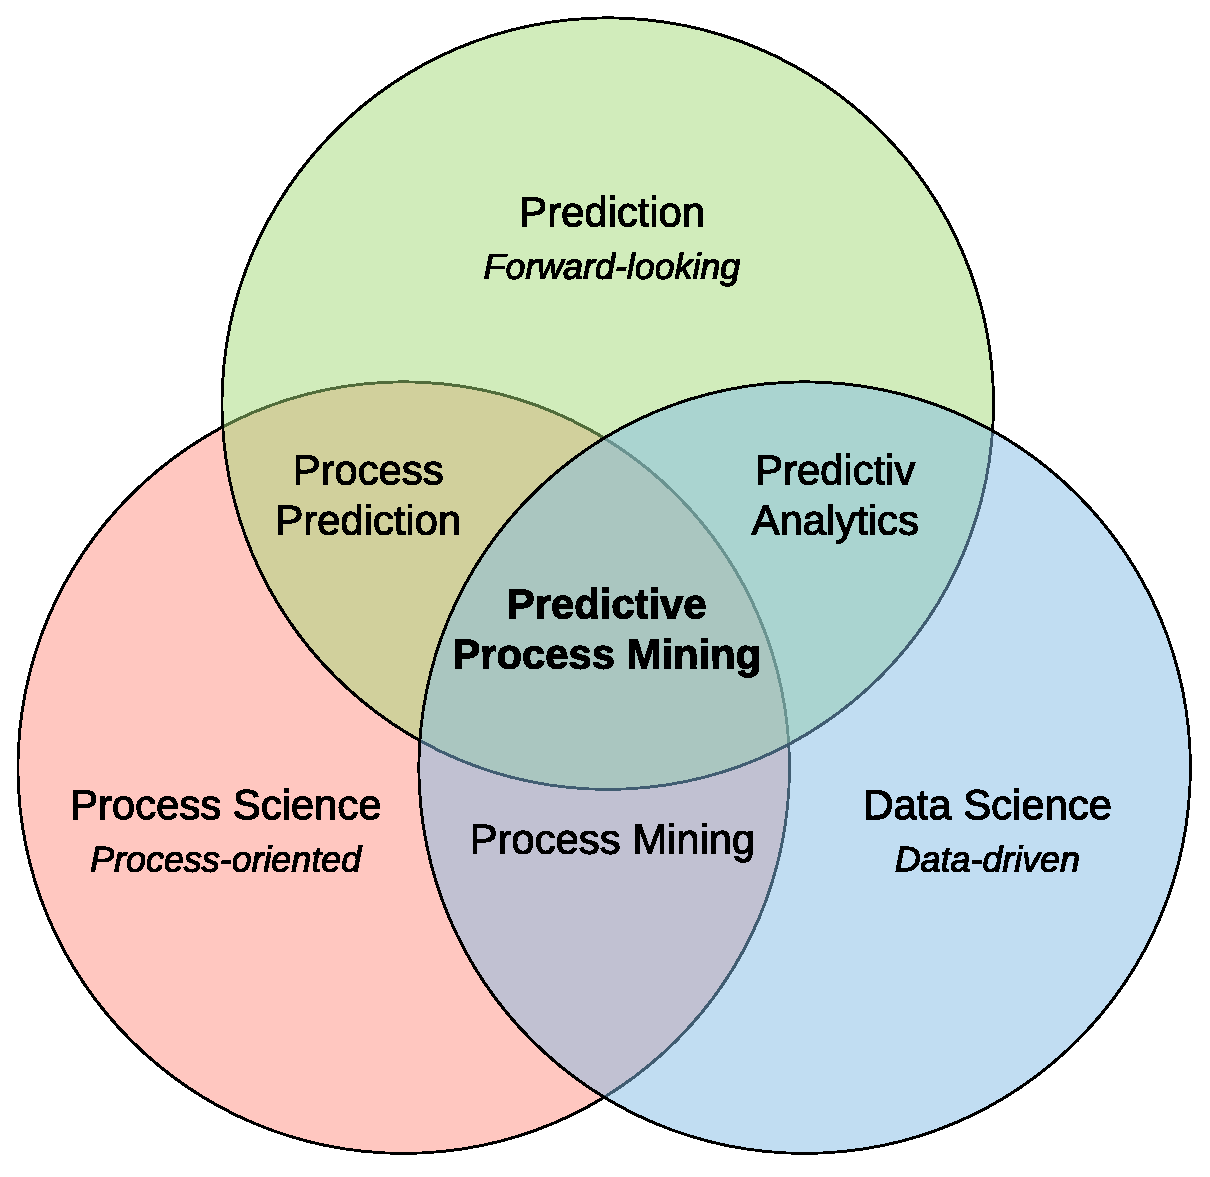
\includegraphics[width=0.5\textwidth]{figures/predictive-process-mining}
	%\caption{Predictive Process Mining combines the concepts of process science, data %science and prediction}
%\end{figure}


\section{Processes and Process Mining}

A \textit{business process} is a collection of activities that are performed in a specific order to archive a goal \cite{DBLP:conf/bpm/AalstAM11}.
A single execution of a process is a \textit{case} or \textit{process instance}, which is identified by a case ID.
Each performed activity belongs to specific case and is completed at a certain time.
For example, a case can be a patient in a hospital, a customer journey or an online order. The time on which an activity for a certain case is performed is specified by a timestamp.
The trinity of case, activity and timestamp is called \textit{event}.
An event can have more attributes, for example resource, costs or transactional information.

\begin{table}[]
	\begin{tabularx}{\textwidth}{@{}lllllll@{}}
		\toprule
		\textbf{ID} & \textbf{Activity}          & \textbf{Timestamp} & \textbf{Resource} & \textbf{Cost} & \textbf{Comment}                                                                                                & \textbf{...} \\ \midrule
		0                & Register patient           & 01.02.2020:14.12   & SYSTEM            & 0             & -                                                                                                               & ...          \\
		& Consultation               & 01.02.2020:14.34   & John Brown, MD    & 24.32         & \begin{tabular}[c]{@{}l@{}}The patient reports persistent\\ nausea.\end{tabular}                                & ...          \\
		& Blood test                 & 01.02.2020:15.12   & Kim Smith         & 14.23         & Tests: Complete blood count                                                                                     & ...          \\
		& Evaluate test result       & 01.02.2020:16.35   & John Brown, MD    & 38.67         & \begin{tabular}[c]{@{}l@{}}No abnormalities in the complete\\ blood count.\end{tabular}                         & ...          \\
		& Release patient            & 01.02.2020:17.24   & SYSTEM            & 0             & -                                                                                                               & ...          \\
		&                            &                    &                   &               &                                                                                                                 &              \\
		1                & Register patient           & 02.02.2020:08.20   & SYSTEM            & 0             & -                                                                                                               & ...          \\
		& Consultation               & 02.02.2020:14.12   & Jana Simpson, MD  & 24.32         & \begin{tabular}[c]{@{}l@{}}Noticeable tachycardia. No chronic pre-existing conditions\\ are known.\end{tabular} & ...          \\
		& MRI & 02.02.2020:14.12   & Sara Taylor, MD   & 352.87        & -                                                                                                               & ...          \\
		& Release patient            & 02.02.2020:14.12   & SYSTEM            & 0             & -                                                                                                               & ...          \\
		&                            &                    &                   &               &                                                                                                                 &              \\
		2                & Register patient           & 02.02.2020:09.08   & SYSTEM            & 0             & -                                                                                                               & ...          \\
		& Consultation               & 02.02.2020:09.14   & Jana Simpson, MD  & 24.32         & \begin{tabular}[c]{@{}l@{}}The patient has severe leg injuries\\ due to a motorcycle accident.\end{tabular}     & ...          \\
		& Patient hospitalized       & 02.02.2020:09.20   & Mike Johnson      & 130.37        & -                                                                                                               & ...          \\
		...              & ...                        & ...                & ...               & ...           & ...                                                                                                             & ...          \\ \bottomrule
	\end{tabularx}
	\caption{Artifical event log of patient treatment in a hospital}
	\label{tab:event-log}
\end{table}

If the execution of a business process is logged by an information system, the resulting event data is called \textit{event log}.
Depending on the format of the event log, it can also contain additional data on case level.
Typical formats for event logs, are comma-separated values (CSV) and eXtensible Event Stream (XES) \cite{DBLP:conf/caise/VerbeekBDA10a}, which can be extracted from databases.
A table-based representation of an artificial event log about patient treatment in a hospital can be seen in Table \ref{tab:event-log}.

Process mining is the discipline that covers all approaches aiming to generate value out of event data.
As an umbrella term, process mining includes or utilizes concepts of business process management, data mining, business process intelligence, big data, workflow management, business process monitoring \cite{DBLP:books/sp/Aalst16} as well as machine learning \cite{DBLP:conf/bpm/VeitGMHT17}.

Traditionally, process mining is divided into a set of subdisciplines mainly process discovery, conformance checking, process enhancement and process analytics \cite{DBLP:conf/caise/EckLLA15}.
Process discovery aims to generate process models out of event data in order to understand a process and enable further analysis.
Conformance checking is about comparing the intended and observed behavior of a process. 
On top of these diagnostic approaches, process enhancement deals with the improvement of processes regarding compliance, performance or complexity.

Finally, process analytics focuses on metric and performance evaluation of processes. Similar to conformance checking, this term is closely related to business process monitoring, a rising subfield enabling the analysis of running business processes in real-time.
Driven by the fast and ongoing development of quantitative prediction methods in data science and machine learning, also prediction-based methods have been applied to event data.
These methods add the forward perspective to business process monitoring and deal with forecasting the future of a running process instance, which is also the main focus of this thesis.


\section{Basic Notations and Sequences}

The set $\mathbb{N}$ denotes the set of all natural numbers $\{1, 2, 3, \dots\}$ and $\mathbb{N}_0 = \mathbb{N} \cup \{0\}$ denotes the set of natural numbers including 0.
The set of natural numbers up to $n$ is noted as $[n] = \{1, 2, \dots, n\} \subset \mathbb{N}$ with [0] = $\emptyset$.

\begin{definition}[Sequence]
		A \textit{sequence} of length $n \in \mathbb{N}_0$ over a set $A$ is an ordered collection of elements defined by function $\sigma \colon [n]\to A$, which assigns each index an element of $A$.
		A sequence  of length $n$ is represented explicitly as $\sigma = \langle a_1, a_2, \dots, a_n\rangle $ with $a_i \in A$ for $1 \leq i \leq n$. In addition, $\langle \rangle$ is the empty sequence of length $0$.
\end{definition}

Given a set $A$, $A^n$ describes the set of all sequences $\langle a_1, a_2, \dots, a_n\rangle$ over $A$ of length $n$.
The set $A^0$ is defined as $\{\langle \rangle\}$, the set that only contains the empty sequence.
The set of all possible sequences over $A$ is given with $A^* = \bigcup\limits_{i\in \mathbb{N}_0} A^i$.

Given sequences $\sigma_1$ and $\sigma_2$, the concatenation of both sequences is denoted by $\sigma_1 \cdot \sigma_2$.
Moreover, the $i$-th element of a sequence $\sigma = \langle a_1, a_2, \dots, a_n\rangle$ is accessed using $\sigma(i)= a_i$ for $1 \leq i \leq n$.
The length of a sequence is denoted by $|\sigma|$.
For a sequence $\sigma=\langle a_1, a_2, \dots, a_n\rangle$, the function
$hd^k(\sigma)= \langle a_1, a_2, \dots, a_k\rangle$ gives the prefix of length $k$ of $\sigma$ and $tl^k(\sigma)= \langle a_{n-k+1}, a_{n-k+2}, \dots, a_n\rangle$ the suffix of length $k$ for $1 \leq k \leq n$.
%Note that $\sigma = hd^k(\sigma) \cdot tl^{n-k+1}(\sigma)$ for corresponding $k$.
%If an element $a_i \in A$ appears in a sequence $\sigma$, we also write $a_i \in \sigma$.

A function $f \colon A \to B$ can be lifted element-wise to sequences over $A$, precisely:
\[
f(\sigma) =
\begin{cases}
\langle \rangle & \text{if $\sigma = \langle \rangle$} \\
\langle f(a_1), f(a_2), \dots, f(a_n)\rangle & \text{else} 
\end{cases}
\]



\section{Events, Traces, Event Logs}

\begin{definition}[Event]
An  \textit{event} is defined by tuple $e = (a,c,t,d_1,\dots, d_m) \in \mathcal{C} \times \mathcal{A}  \times \mathcal{T} \times \mathcal{D}_1 \times \dots \times \mathcal{D}_m =  \mathcal{E}$ where  $c \in \mathcal{C} $ is the case ID, $a \in \mathcal{A}$ is the executed activity and $t \in \mathcal{T}$ is the timestamp of the event.
Furthermore, each event contains a fixed number $m \in \mathbb{N}_0$ of additional attributes $d_1 \dots d_m$ in their corresponding domains $\mathcal{D}_1, \dots , \mathcal{D}_m$.
In case that no additional attribute data is given ($m = 0$) the event space $\mathcal{E}$ (set of all possible events) is reduced to $\mathcal{C} \times \mathcal{A}  \times \mathcal{T}$.
\end{definition}

Each attribute $d \in \mathcal{D}$ of an event (including activity, timestamp and case ID) can be accessed by a projection function $\pi_D \colon \mathcal{E} \to \mathcal{D}$.
For example, the activity $a$ of an event $e$ is retrieved by $\pi_\mathcal{A}(e) = a$.

Throughout this thesis,  $\mathcal{C} = \mathbb{N}_0$, $|\mathcal{A}| < \infty$ and $ \mathcal{T} = \mathbb{R}$ is assumed, where $t \in \mathcal{T}$ is given in Unix time, precisely the number of seconds since 00:00:00 UTC on 1 January 1970 minus the applied leap seconds.
Each additional attribute is assumed to be numerical, categorical or textual, i.e. $\mathcal{D}_i = \mathbb{R}$, $|\mathcal{D}_i| < \infty$ or $\mathcal{D}_i = \Sigma^\ast$  for $1 \leq i \leq m$ and some fixed Alphabet $\Sigma$.

\begin{definition}[Trace]
	A \textit{trace} is a finite and non-empty sequence of events $\sigma = \langle e_1, e_2, \dots\rangle \in  \mathcal{E}^\ast$ with increasing timestamps, i.e. $\pi_\mathcal{T} (e_i) < \pi_\mathcal{T} (e_j) $ for $1 \leq i < j \leq |\sigma|$.
\end{definition}


By lifting the projection functions to sequences a trace can be transformed into a sequence of attributes by applying the projection function to the trace.
For example, $\pi_\mathcal{A}(\sigma)$ gives the sequence of the activities of the events in $\sigma$.

\begin{definition}[Event log]
	An \textit{event log} $\eventlog = \{ \sigma_1, \sigma _2, \dots, \sigma_k \}$ is a set of traces, where each event of a trace is unique in the log and all events of a trace share a case IDs, which is unique per trace.
\end{definition}

\section{Text Mining}

\textit{Text mining} describes all techniques to generate value out of unstructured or semi-structured textual data.
It combines concepts of natural language processing, machine learning and data mining \cite{DBLP:journals/coling/Mihalcea08}.
The base object in text mining is a \textit{document} containing textual data.
The text can be completed unstructured, i.e. it does not conform to a pre-defined data model, or semi-structured, like in an e-mail, where text information is assigned to sender, subject, message etc.
A collection of documents is called \textit{text corpus}, which forms the basis for many text mining techniques.

In order to derive a mathematical representation of the text data that can be interpreted by a computer, a text model has to be build using the text corpus.
Popular text models are Bag-of-words, Bag-of-n-gram, Paragraph vector (a.k.a. Doc2Vec) \cite{DBLP:conf/icml/LeM14} and Latent Dirichlet Allocation \cite{DBLP:journals/jmlr/BleiNJ03}.
Most models require a text normalization step, where the text is cleaned from linguistic variation as well as meaningless words and symbols \cite{DBLP:books/lib/JurafskyM09}.

\section{Supervised Learning}

In \textit{supervised learning} an unknown function is learned (i.e. approximated) from a set of example input-output pairs \cite{DBLP:books/daglib/0023820}.
In contrast, \textit{unsupervised learning} does not require examples pattern and is about finding pattern in the data. 
An input instance is usually described by a set of feature variables $X$ and the output is defined by a target variable $y$.
If the target variable $y$ is continuous, we refer to this as a regression problem, if however it is discrete variable with a finite range of values, the learning problem is called classification problem.
Given a \textit{training set} of input-output pairs $\{(X_1, y_1), (X_2, y_2), \dots, (X_m,y_m)\}$, that were generated from an unknown function $y = f(X)$, the goal is to approximate a hypothesis function $h(X)$, which is close to f(X), i.e. $h(X) \approx f(X)$.

The challenge in supervised learning is to generalize from the training set of input-output pairs in such a way, that the learned hypothesis function $h(x)$ can also successfully predict the target variable for unseen problem instances.
In order to evaluate a hypothesis, the function is tested on a separate \textit{test set} of input-output pairs, which has not been used for the construction of $h(X)$.

A hypothesis generalizes well, if its prediction performance is high on the training set as well as on test set.
However, if the prediction performance is high on the training set, but not reliable on unseen data, the hypothesis \textit{overfits} the training data.
In this case, the model complexity, i.e. the number of parameters is higher than justified by the true function. 
In contrast, if the model is too simple to fit any data from training set, the hypothesis is \textit{underfitting}.

In many real-world applications, the true function $f(X)$ is stochastic, i.e. we need to estimate a conditional probability function $P(Y | X)$ (classification problem) or a conditional expectation $E(Y | X)$ (regression problem) for prediction.
Therefore, the prediction accuracy is always limited by the variation of the true distribution.




\section{Long Short-Term Memory Networks}

Long short-term memory (LSMT) is an advanced recurrent neural network architecture for sequential data originally presented by \citeauthor{DBLP:journals/neco/HochreiterS97} in \citeyear{DBLP:journals/neco/HochreiterS97}  \cite{DBLP:journals/neco/HochreiterS97}.
This approach addresses the well-known vanishing and exploding gradient problem \cite{DBLP:conf/icml/PascanuMB13}  of traditional recurrent neural networks by introducing more complex LSTM cells as hidden units.
The proposed architecture has been improved several times \cite{DBLP:journals/neco/GersSC00} \cite {DBLP:journals/tnn/GreffSKSS17} and considered as one of the most successful recurrent neural network models.
Although LSTM networks have been available for a long time, the breakthrough of this technology is dated around 2016 after many success stories of LSTM in combination with large data sets and GPU hardware have been reported for sequence to sequence tasks like text translation \cite{DBLP:journals/corr/WuSCLNMKCGMKSJL16}.

Gated recurrent units (GRU) \cite{DBLP:conf/emnlp/ChoMGBBSB14} are the competing gating mechanism by \citeauthor{DBLP:conf/emnlp/ChoMGBBSB14} that have fewer parameters and perform similar to LSTM.
However, more recent studies show, that LSTM outperforms GRU consistently in neural machine translation tasks \cite{DBLP:journals/corr/BritzGLL17}.

A simple feedforward neural networks consists of an input layer, arbitrarily many hidden layers and an output layer, where each layer consists of neurons that compute and output the weighted sum of the cells of the previous layer that has been passed to an non-linear activation function \cite{DBLP:journals/nn/Schmidhuber15}.
These networks can learn and compute complex functions in supervised learning settings, where input and output pattern are provided.
The network computes a loss function for each training pattern and adjusts its weights with gradient descents using a back-propagation algorithm in order to minimize the loss function \cite{rumelhart1986learning}.

Recurrent neural networks extend traditional feed forward networks with backfeeding connections between hidden layers.
This enables the network to keep a state across inputs and allows the neural network to process arbitrarily long sequences of input data while learning temporal dependencies.

In LTSM networks the layers are replaced by more complex LSTM modules, where each module contains four different sublayers.
The module uses as input the state $\vec{c}_{t-1}$ and the hidden output $\vec{h}_{t-1}$ of the module in the previous time step as well as the output of the previous layer $\vec{x}_t$ to compute a new cell state $\vec{c}_{t}$ and a (hidden) output $\vec{h}_{t}$.

\begin{figure}[htbp!]
	\centering
	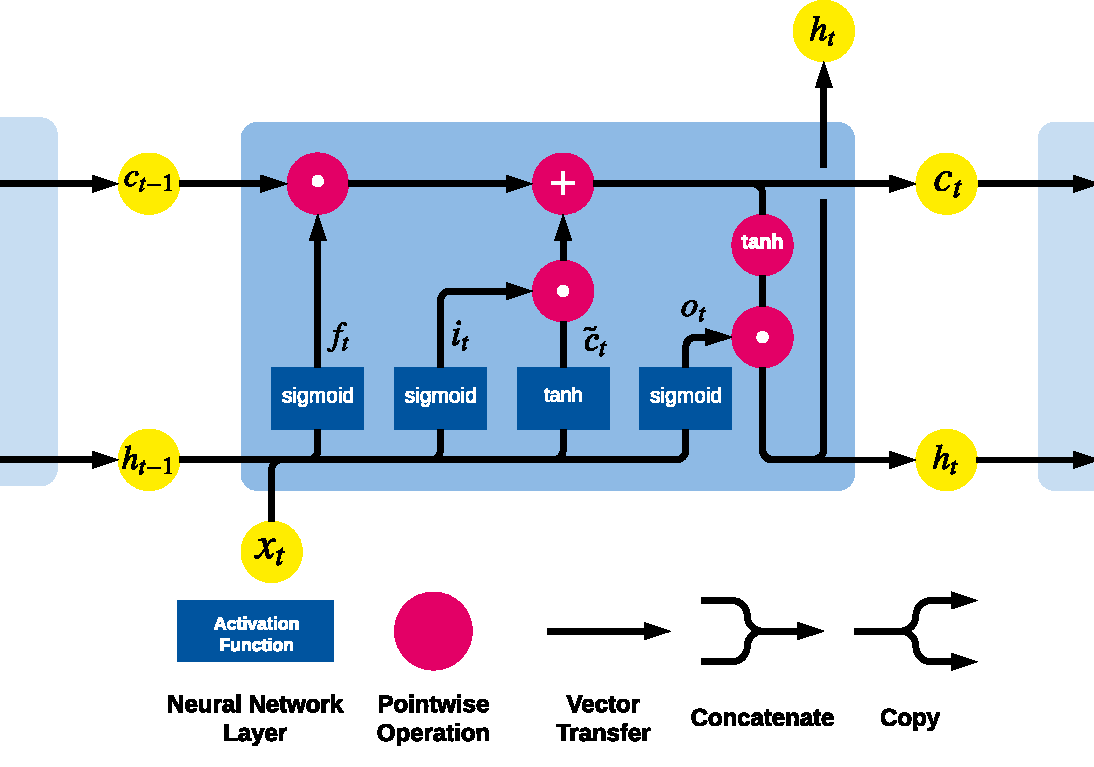
\includegraphics[width=0.8\textwidth]{figures/lstm-module}
	\caption{An LSTM module with four sublayers that manipulate the cell state and compute the module's output. Graphic adapted from \cite{lstm-blog}.}
	\label{fig:lstm-module}
\end{figure}


The input vector $\vec{x}_t$ is concatenated with the previous hidden output $\vec{h}_{t-1}$ and fed to four neural network layers, which are designed to decide what part of the cell state will remain (forget gate $\vec{f}_t$), how it is updated (update gate $\vec{i}_t$ and $\vec{\bar{c}}_t$) and what the output of the layer will be (output gate $\vec{o}_t$ leading to $\vec{h}_t$).
The sublayer apply $\text{sigmoid}(x) = \frac{1}{1+\exp({-x})}$ or $\tanh(x) = \frac{\exp({x}) - \exp({-x})}{\exp({x}) + \exp({-x})}$ activation functions elementwise, leading to the following equations:

\begin{equation*}
	\vec{f}_t = \text{sigmoid}(\vec{W}_f \cdot (\vec{h}_{t-1}, \vec{x}_t) + \vec{b}_f)
\end{equation*}

\begin{equation*}
	\vec{i}_t =  \text{sigmoid} (\vec{W}_i \cdot (\vec{h}_{t-1}, \vec{x}_t) + \vec{b}_i)
\end{equation*}

\begin{equation*}
	\vec{\bar{c}}_t = \tanh (\vec{W}_c \cdot (\vec{h}_{t-1}, \vec{x}_t) + \vec{b}_c)
\end{equation*}

\begin{equation*}
	\vec{o}_t =  \text{sigmoid} (\vec{W}_o \cdot (\vec{h}_{t-1}, \vec{x}_t) + \vec{b}_o)
\end{equation*}

$\vec{W}_f$, $\vec{W}_i$, $\vec{W}_c$ and $\vec{W}_o$ are the sublayer's learned weights and $\vec{b}_f$, $\vec{b}_i$, $\vec{b}_c$ and $\vec{b}_o$ are the corresponding biases.

The new cell state $\vec{c}_t$ is then a combination of the old cell state $\vec{c}_{t-1}$ and the result of the update gate $\vec{\bar{c}}_t$, where the layer computations $\vec{f}_t$ and $\vec{i}_t$ determine the proportions by a pointwise multiplication ($\odot$) with the cell states.

\begin{equation*}
	\vec{c}_t = f_t \odot \vec{c}_{t-1} + \vec{i}_t \odot \vec{\bar{c}}_t
\end{equation*}

The result of the output gate $\vec{o}_t$ is pointwise multiplied with the tanh-activated new cell state to calculate the hidden output $\vec{h}_t$ of the module.

\begin{equation*}
	\vec{h}_t = \vec{o}_t \odot \tanh(\vec{c}_t )
\end{equation*}

LSTM networks are able to backpropagate a more stable error with this gating mechanism, such that these networks are much more capable of learning complex functions for sequences compared to standard recurrent neural networks.